\sectionthree{C++ STL unordered map}
\begin{python0}
from solutions import *; clear()
\end{python0}

The C++ STL contains the \verb!unordered_map! class template
which is a hashtable.
You will need to compile your code with at least C++11:
\begin{console}
g++ *.cpp -std=c++11
\end{console}
\verb!unordered_map! uses open hashing (separate chaining), i.e., 
i.e., it's an array of linked list of key-value pairs.
The class:
\begin{console}
std::unordered_map< X, Y >
\end{console}
assumes that type (or class) \verb!X! has
\verb!operator==()!
(for the obvious reason).
Also, each (key, value) pair in the hashtable
is a \verb!std::pair< X, Y >! object
(you can think of such an object as a 2-tuple).
If \verb!pair! is a
\verb!std::pair< X, Y >! value,
then the first value is \verb!pair.first! has type \verb!X!
and the second value is \verb!pair.second! of type \verb!Y!.

To add a key-value pair $(k,v)$ into a
\verb!std::unordered_map< X, Y >! object \verb!h!, you do either
\begin{console}
h.insert({k, v}); // check if error
\end{console}
or
\begin{console}
h[k] = v;
\end{console}
Both methods in the above work in the same way if \verb!k! is not in \verb!h!.
If \verb!k! is in \verb!h!, then
\verb!h.insert({k, v})! will give you an exception
while
\verb!h[k] = v! will update the value of \verb!k! with \verb!v!.

\verb!h.find(k)! will return an iterator.
The iterator will equal \verb!h.end()! if \verb!k! is not found.
Otherwise it will point to the
\verb!std::pair! object with the given key (as first value).
\begin{console}
auto p = h.find(k);
std::cout << (p == h.end() ? "not found\n" : "found\n");  
\end{console}

As mentioned above C++ unordered map is implemented using open address hashtable,
i.e., it's an array of linked list of key-value pairs.
Each linked list is also called a bucket.
Besides that, the (key, value) pairs on in buckets
where each bucket has a linked list of (key, value) pairs.
If \verb!h! is an unordered map,
then \verb!h.bucket(k)! is \verb!i! where
\verb!k! is found in the \verb!i!--th bucket
where \verb!i! = 0, ..., \verb!h.bucket_count() - 1!.
You can get an iterator to run through a bucket (not the whole hashtable).
The following prints all the key-value pairs in bucket $i$:
\begin{console}
for (typename T::const_local_iterator p = h.begin(i);
     p != h.end(i); ++p)
{
    std::cout << p->first << ": " << p->second << "  ";
}
\end{console}

You also have iterators that runs through all the buckets, i.e., the whole hashtable:
\begin{console}[fontsize=\footnotesize]
for (typename std::unordered_map< X, Y >::const_iterator p = h.begin();
     p != h.end(); ++p)
{
    std::cout << p->first << ": " << p->second << "  ";
}
\end{console}

Study the following program carefully.

\begin{center}
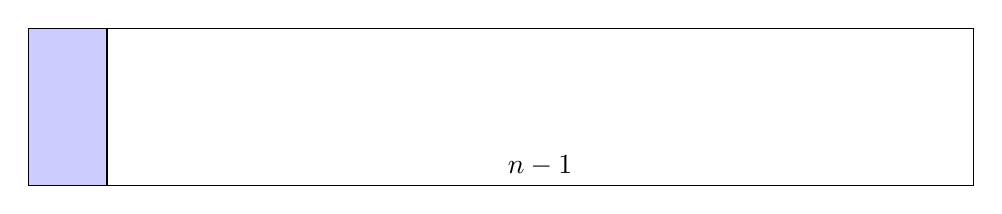
\begin{tikzpicture}

\draw (6.0, 1.0)
  node[draw, , , color=black,
       rounded corners=0cm, inner sep=0cm] {

\begin{minipage}[t][2cm]{12cm}
\mbox{}

\end{minipage}

};
\draw (0.5, 1.0)
  node[fill=blue!20!white,rounded corners=0cm,inner sep=0cm] {

\begin{minipage}[t][2cm]{1cm}
\mbox{}

\end{minipage}

};
\draw (0.5, 1.0)
  node[draw, , , color=black,
       rounded corners=0cm, inner sep=0cm] {

\begin{minipage}[t][2cm]{1cm}
\mbox{}

\end{minipage}

};
\draw (6.5, 0.25)
  node[draw=none, line width=0cm, , color=black,
       rounded corners=0cm, inner sep=0cm] {

\begin{minipage}[t][0.1cm]{0.1cm}
\mbox{}

\end{minipage}

};\draw (6.5, 0.25) node[color=black] {$n - 1$};
\end{tikzpicture}

\end{center}


\vspace{-0.1cm}
{\small
\VerbatimInput[frame=single]{main23.cpp}
\VerbatimInput[frame=single]{out23.txt}
}

For convenience, I'm going to put some of the above code
into \verb!Height.h!:

\begin{center}
\begin{tikzpicture}

\fill[blue!10] (0.0, 0.0) circle (0.3);
\node [line width=0.03cm,black,minimum size=0.57cm,draw,circle] at (0.0,0.0)(a){};\draw (0.0, 0.0) node[color=black] {$a$};
\fill[blue!10] (-2.0, -1.0) circle (0.3);
\node [line width=0.03cm,black,minimum size=0.57cm,draw,circle] at (-2.0,-1.0)(b){};\draw (-2.0, -1.0) node[color=black] {$b$};
\fill[blue!10] (2.0, -1.0) circle (0.3);
\node [line width=0.03cm,black,minimum size=0.57cm,draw,circle] at (2.0,-1.0)(d){};\draw (2.0, -1.0) node[color=black] {$d$};
\fill[blue!10] (-3.0, -2.0) circle (0.3);
\node [line width=0.03cm,black,minimum size=0.57cm,draw,circle] at (-3.0,-2.0)(e){};\draw (-3.0, -2.0) node[color=black] {$e$};
\fill[blue!10] (-1.0, -2.0) circle (0.3);
\node [line width=0.03cm,black,minimum size=0.57cm,draw,circle] at (-1.0,-2.0)(f){};\draw (-1.0, -2.0) node[color=black] {$f$};
\fill[blue!10] (1.0, -2.0) circle (0.3);
\node [line width=0.03cm,black,minimum size=0.57cm,draw,circle] at (1.0,-2.0)(m){};\draw (1.0, -2.0) node[color=black] {$m$};
\fill[blue!10] (3.0, -2.0) circle (0.3);
\node [line width=0.03cm,black,minimum size=0.57cm,draw,circle] at (3.0,-2.0)(o){};\draw (3.0, -2.0) node[color=black] {$o$};
\fill[blue!10] (-3.5, -3.0) circle (0.3);
\node [line width=0.03cm,black,minimum size=0.57cm,draw,circle] at (-3.5,-3.0)(k){};\draw (-3.5, -3.0) node[color=black] {$k$};
\fill[blue!10] (-2.5, -3.0) circle (0.3);
\node [line width=0.03cm,black,minimum size=0.57cm,draw,circle] at (-2.5,-3.0)(l){};\draw (-2.5, -3.0) node[color=black] {$l$};
\fill[blue!10] (3.5, -3.0) circle (0.3);
\node [line width=0.03cm,black,minimum size=0.57cm,draw,circle] at (3.5,-3.0)(j){};\draw (3.5, -3.0) node[color=black] {$j$};\draw[line width=0.03cm,black,->,>=triangle 60] (a) to  (b);
\draw[line width=0.03cm,black,->,>=triangle 60] (a) to  (d);
\draw[line width=0.03cm,black,->,>=triangle 60] (b) to  (e);
\draw[line width=0.03cm,black,->,>=triangle 60] (b) to  (f);
\draw[line width=0.03cm,black,->,>=triangle 60] (d) to  (m);
\draw[line width=0.03cm,black,->,>=triangle 60] (d) to  (o);
\draw[line width=0.03cm,black,->,>=triangle 60] (e) to  (k);
\draw[line width=0.03cm,black,->,>=triangle 60] (e) to  (l);
\draw[line width=0.03cm,black,->,>=triangle 60] (o) to  (j);
\end{tikzpicture}

\end{center}


\vspace{-0.1cm}
{\small
\VerbatimInput[frame=single]{Height.h}
}

Note that the \verb!reserve()! method (to change the number of
bucket) asks for 641 buckets, but you might get a number $\geq 641$.






{\footnotesize
\begin{tabular}{|p{0.4\textwidth}|p{0.55\textwidth}|}
  \hline
  xxx  & yyy
  \\
  \hline \hline
  \texttt{std::unordered\_map< K, V > h} & \texttt{h} is a hashtable of \texttt{std::pair< K, V >} \\ \hline 
  \texttt{h.reserve(n)}                &                                                           \\ \hline 
  \texttt{h.insert(\{k, v\})}          & Add \texttt{(k, v)} to \texttt{h}. If \verb!k! is already in \verb!h!, \verb!h! is not changed. \\ \hline
  \texttt{h[k]} = v                    & If \verb!k! is in \verb!h!, its value is changed to \verb!v!. If \verb!k! is not found, \verb!(k,v)! is inserted. \\ \hline
  \texttt{h.erase(k)}                  & Remove \verb!k! from \verb!h!.                            \\ \hline
  \texttt{h.begin()}                   &                                                           \\ \hline
  \texttt{h.end()}                     &                                                           \\ \hline
  \texttt{h.find(k)}                   & Return \texttt{std::unordered\_map< X, Y >::iterator} \\ \hline
  \texttt{h.bucket\_count()}           &                                                           \\ \hline
  \texttt{h.bucket(i)}                 &                                                           \\ \hline
  \texttt{h.begin(i)}                  &                                                           \\ \hline

  \texttt{h.end(i)}                    &                                                           \\ \hline
  \texttt{h.size()}                    & Number of key-value pairs in \verb!h!                     \\ \hline
  \texttt{h.load\_factor()}            &                                                           \\ \hline
  \texttt{h.max\_load\_factor()}       &                                                           \\ \hline
\end{tabular}
}

\subsection{Hash function}

Note that in the above examples, when we use \verb!std::unordered_map!,
we don't have to say how to hash the keys.
That's because \verb!std::unordered_map! use the built-in
\verb!std::hash!.
Go ahead and run this:
\begin{center}
\begin{tikzpicture}

\fill[blue!10] (0.0, 0.0) circle (0.3);
\node [line width=0.03cm,black,minimum size=0.57cm,draw,circle] at (0.0,0.0)(a){};\draw (0.0, 0.0) node[color=black] {$a$};
\fill[blue!10] (-2.0, -1.0) circle (0.3);
\node [line width=0.03cm,black,minimum size=0.57cm,draw,circle] at (-2.0,-1.0)(b){};\draw (-2.0, -1.0) node[color=black] {$b$};
\fill[blue!10] (2.0, -1.0) circle (0.3);
\node [line width=0.03cm,black,minimum size=0.57cm,draw,circle] at (2.0,-1.0)(d){};\draw (2.0, -1.0) node[color=black] {$d$};
\fill[blue!10] (-3.0, -2.0) circle (0.3);
\node [line width=0.03cm,black,minimum size=0.57cm,draw,circle] at (-3.0,-2.0)(e){};\draw (-3.0, -2.0) node[color=black] {$e$};
\fill[blue!10] (-1.0, -2.0) circle (0.3);
\node [line width=0.03cm,black,minimum size=0.57cm,draw,circle] at (-1.0,-2.0)(f){};\draw (-1.0, -2.0) node[color=black] {$f$};
\fill[blue!10] (1.0, -2.0) circle (0.3);
\node [line width=0.03cm,black,minimum size=0.57cm,draw,circle] at (1.0,-2.0)(m){};\draw (1.0, -2.0) node[color=black] {$m$};
\fill[blue!10] (3.0, -2.0) circle (0.3);
\node [line width=0.03cm,black,minimum size=0.57cm,draw,circle] at (3.0,-2.0)(j){};\draw (3.0, -2.0) node[color=black] {$j$};
\fill[blue!10] (-3.5, -3.0) circle (0.3);
\node [line width=0.03cm,black,minimum size=0.57cm,draw,circle] at (-3.5,-3.0)(k){};\draw (-3.5, -3.0) node[color=black] {$k$};
\fill[blue!10] (-2.5, -3.0) circle (0.3);
\node [line width=0.03cm,black,minimum size=0.57cm,draw,circle] at (-2.5,-3.0)(l){};\draw (-2.5, -3.0) node[color=black] {$l$};\draw[line width=0.03cm,black,->,>=triangle 60] (a) to  (b);
\draw[line width=0.03cm,black,->,>=triangle 60] (a) to  (d);
\draw[line width=0.03cm,black,->,>=triangle 60] (b) to  (e);
\draw[line width=0.03cm,black,->,>=triangle 60] (b) to  (f);
\draw[line width=0.03cm,black,->,>=triangle 60] (d) to  (m);
\draw[line width=0.03cm,black,->,>=triangle 60] (d) to  (j);
\draw[line width=0.03cm,black,->,>=triangle 60] (e) to  (k);
\draw[line width=0.03cm,black,->,>=triangle 60] (e) to  (l);
\end{tikzpicture}

\end{center}


{\small
\VerbatimInput[frame=single]{main.cpp}
}

\begin{center}
\begin{tikzpicture}[>=triangle 60,shorten >=0.5pt,node distance=2cm,auto,initial text=, double distance=2pt]
\node[state,initial] (A) at (  0,  0) {$q_0$};
\node[state] (B) at (  4,  0) {$q_1$};
\node[state,accepting] (D) at (  8,  0) {$q_3$};
\node[state] (C) at (  4, -4) {$q_2$};

\path[->]
(A) edge [loop above] node {$a$} ()
(A) edge [bend left=0,pos=0.5,above] node {$\epsilon$} (B)
(A) edge [bend left=0,pos=0.5,above] node {$a$} (C)
(B) edge [bend left=0,pos=0.5,above] node {$b$} (D)
(C) edge [bend left=0,pos=0.5] node {$a,\epsilon$} (B)
(D) edge [bend left=0,pos=0.5] node {$a,b$} (C)

;
\end{tikzpicture}
\end{center}
    

The return value of \verb!std::hash! is a \verb!size_t! value,
which is like an unsigned integer value
that is usually takes up 32 or 64 bits.

For \verb!int! and \verb!unsigned int! variable
\verb!x!, note that \verb!std::hash(x)!
is the same as \verb!(size_t)(x)!.
For \verb!bool! and \verb!char! values, they are typecasted to
\verb!size_t! values.
For double and string
So \verb!std::hash! knows how to has values of
the following types:
\verb!int!, \verb!double!, \verb!char!, \verb!std::string!.
But what if you want to hash values of other types?

You can define your own hash function for
\verb!X! values where \verb!X! is the first
type (the key type) of the unordered map.
There are several ways to do this.

\textsc{Method 1.}
One way is to create a class or struct where objects are function
objects (i.e., they have \verb!operator()!) that
returns an \verb!size_t! or unsigned int when given a value of type \verb!X!.
You then include this class as the third type parameter
for \verb!unordered_map!:

\begin{center}
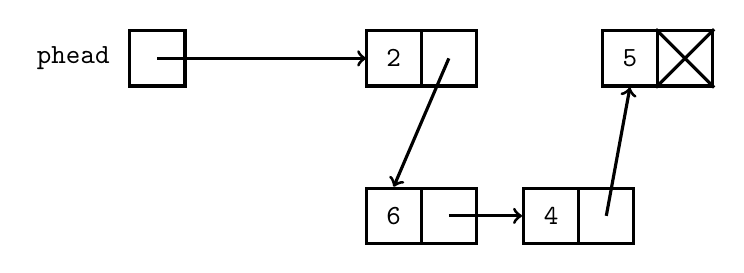
\begin{tikzpicture}

\draw (0.35, 0.35)
  node[draw, line width=0.04cm, , color=black,
       rounded corners=0cm, inner sep=0cm] {

\begin{minipage}[t][0.7cm]{0.7cm}
\mbox{}

\end{minipage}

};\draw (0.35, 0.35) node[color=black] {{\texttt{2}}};
\draw (1.0499999999999998, 0.35)
  node[draw, line width=0.04cm, , color=black,
       rounded corners=0cm, inner sep=0cm] {

\begin{minipage}[t][0.7cm]{0.7cm}
\mbox{}

\end{minipage}

};\draw (1.0499999999999998, 0.35) node[color=black] {{\texttt{}}};
\draw (0.35, -1.65)
  node[draw, line width=0.04cm, , color=black,
       rounded corners=0cm, inner sep=0cm] {

\begin{minipage}[t][0.7cm]{0.7cm}
\mbox{}

\end{minipage}

};\draw (0.35, -1.65) node[color=black] {{\texttt{6}}};
\draw (1.0499999999999998, -1.65)
  node[draw, line width=0.04cm, , color=black,
       rounded corners=0cm, inner sep=0cm] {

\begin{minipage}[t][0.7cm]{0.7cm}
\mbox{}

\end{minipage}

};\draw (1.0499999999999998, -1.65) node[color=black] {{\texttt{}}};
\draw (2.35, -1.65)
  node[draw, line width=0.04cm, , color=black,
       rounded corners=0cm, inner sep=0cm] {

\begin{minipage}[t][0.7cm]{0.7cm}
\mbox{}

\end{minipage}

};\draw (2.35, -1.65) node[color=black] {{\texttt{4}}};
\draw (3.0500000000000003, -1.65)
  node[draw, line width=0.04cm, , color=black,
       rounded corners=0cm, inner sep=0cm] {

\begin{minipage}[t][0.7cm]{0.7cm}
\mbox{}

\end{minipage}

};\draw (3.0500000000000003, -1.65) node[color=black] {{\texttt{}}};
\draw (3.35, 0.35)
  node[draw, line width=0.04cm, , color=black,
       rounded corners=0cm, inner sep=0cm] {

\begin{minipage}[t][0.7cm]{0.7cm}
\mbox{}

\end{minipage}

};\draw (3.35, 0.35) node[color=black] {{\texttt{5}}};
\draw (4.05, 0.35)
  node[draw, line width=0.04cm, , color=black,
       rounded corners=0cm, inner sep=0cm] {

\begin{minipage}[t][0.7cm]{0.7cm}
\mbox{}

\end{minipage}

};\draw (4.05, 0.35) node[color=black] {{\texttt{}}};\draw[line width=0.04cm,black,->] (1.05,0.35) to  (0.35,-1.28);
\draw[line width=0.04cm,black,->] (1.05,-1.65) to  (1.98,-1.65);
\draw[line width=0.04cm,black,->] (3.05,-1.65) to  (3.35,-0.02);
\draw[line width=0.04cm,black] (3.68,0.72) to  (4.42,-0.02);
\draw[line width=0.04cm,black] (4.42,0.72) to  (3.68,-0.02);

\draw (-2.65, 0.35)
  node[draw, line width=0.04cm, , color=black,
       rounded corners=0cm, inner sep=0cm] {

\begin{minipage}[t][0.7cm]{0.7cm}
\mbox{}

\end{minipage}

};\draw (-2.65, 0.35) node[color=black] {{\texttt{}}};\draw[line width=0.04cm,black,->] (-2.65,0.35) to  (0,0.35);

\draw (-3.7199999999999998, 0.35)
  node[draw, line width=0.04cm, , color=white,
       rounded corners=0cm, inner sep=0cm] {

\begin{minipage}[t][0.1cm]{0.1cm}
\mbox{}

\end{minipage}

};\draw (-3.7199999999999998, 0.35) node[color=black] {{\texttt{phead}}};
\end{tikzpicture}

\end{center}


\vspace{-0.1cm}
{\small
\VerbatimInput[frame=single]{main.cpp}
\VerbatimInput[frame=single]{out.txt}
}

\textsc{Method 2.}
Here's a second method to create a hash function to be used
by \verb!unordered_map!.
This method is not as flexible as the above method
and can only be used when the hashing is performed
on a class that is not yet defined.
Suppose you have a class \verb!vec2d!
where \verb!operator==! is defined.
Each \verb!vec2d! has two \verb!double! members
that can be accessed by public methods
\verb!vec2d::x()! and
\verb!vec2d::y()!
Note that \verb!std::hash< double >! is already defined.
Basically I want to create a hash function on \verb!vec2d! objects
using \verb!std::hash< double >!.

I can do this:
\begin{center}
\begin{tikzpicture}
\draw[line width=0.03cm,red,<->] (7) to [bend left=90]  (8);

\fill[blue!10] (0.0, 0.0) circle (0.35);
\node [line width=0.03cm,black,minimum size=0.6699999999999999cm,draw,circle] at (0.0,0.0)(10){};\draw (0.0, 0.0) node[color=black] {\texttt{10}};
\fill[blue!10] (-0.95, -1.0) circle (0.35);
\node [line width=0.03cm,black,minimum size=0.6699999999999999cm,draw,circle] at (-0.95,-1.0)(5){};\draw (-0.95, -1.0) node[color=black] {\texttt{5}};
\fill[blue!10] (0.95, -1.0) circle (0.35);
\node [line width=0.03cm,black,minimum size=0.6699999999999999cm,draw,circle] at (0.95,-1.0)(7){};\draw (0.95, -1.0) node[color=black] {\texttt{7}};
\fill[blue!10] (-1.43, -2.0) circle (0.35);
\node [line width=0.03cm,black,minimum size=0.6699999999999999cm,draw,circle] at (-1.43,-2.0)(2){};\draw (-1.43, -2.0) node[color=black] {\texttt{2}};
\fill[blue!10] (-0.47, -2.0) circle (0.35);
\node [line width=0.03cm,black,minimum size=0.6699999999999999cm,draw,circle] at (-0.47,-2.0)(1){};\draw (-0.47, -2.0) node[color=black] {\texttt{1}};
\fill[blue!10] (0.47, -2.0) circle (0.35);
\node [line width=0.03cm,black,minimum size=0.6699999999999999cm,draw,circle] at (0.47,-2.0)(0){};\draw (0.47, -2.0) node[color=black] {\texttt{0}};
\fill[blue!10] (1.43, -2.0) circle (0.35);
\node [line width=0.03cm,black,minimum size=0.6699999999999999cm,draw,circle] at (1.43,-2.0)(8){};\draw (1.43, -2.0) node[color=black] {\texttt{8}};\draw[line width=0.03cm,black] (10) to  (5);
\draw[line width=0.03cm,black] (10) to  (7);
\draw[line width=0.03cm,black] (5) to  (2);
\draw[line width=0.03cm,black] (5) to  (1);
\draw[line width=0.03cm,black] (7) to  (0);
\draw[line width=0.03cm,black] (7) to  (8);
\end{tikzpicture}

\end{center}


\vspace{-0.1cm}
{\small
\VerbatimInput[frame=single]{main.cpp}
}
In this case, note that the class
\verb!std::unordered_map< vec2d, double >!
does not require us to include the hash.
That's because we have extended \verb!std::hash!
to be able to handle \verb!vec2d! objects,
which is used by default.

Note that this method is not as flexible as the first method.
This is because you cannot, for instance, have two different
\verb!std::hash< std::string >!.


\subsection{Size}

Now I'm going to resize to a smaller size:

\begin{center}
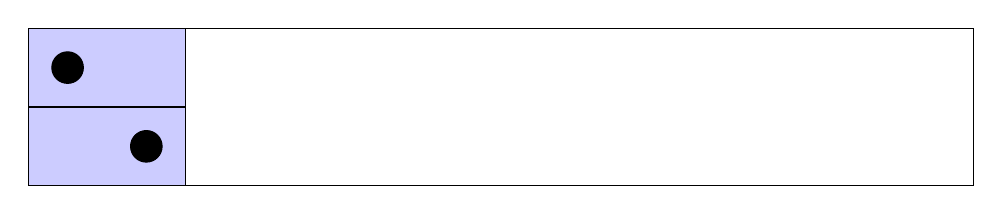
\begin{tikzpicture}

\draw (6.0, 1.0)
  node[draw, , , color=black,
       rounded corners=0cm, inner sep=0cm] {

\begin{minipage}[t][2cm]{12cm}
\mbox{}

\end{minipage}

};
\draw (1.0, 1.5)
  node[fill=blue!20!white,rounded corners=0cm,inner sep=0cm] {

\begin{minipage}[t][1cm]{2cm}
\mbox{}

\end{minipage}

};
\draw (1.0, 1.5)
  node[draw, , , color=black,
       rounded corners=0cm, inner sep=0cm] {

\begin{minipage}[t][1cm]{2cm}
\mbox{}

\end{minipage}

};
\fill[black] (0.5, 1.5) circle (0.2);
\draw[black] (0.5, 1.5) circle (0.2);
\draw (1.0, 0.5)
  node[fill=blue!20!white,rounded corners=0cm,inner sep=0cm] {

\begin{minipage}[t][1cm]{2cm}
\mbox{}

\end{minipage}

};
\draw (1.0, 0.5)
  node[draw, , , color=black,
       rounded corners=0cm, inner sep=0cm] {

\begin{minipage}[t][1cm]{2cm}
\mbox{}

\end{minipage}

};
\fill[black] (1.5, 0.5) circle (0.2);
\draw[black] (1.5, 0.5) circle (0.2);
\end{tikzpicture}

\end{center}


\vspace{-0.1cm}
{\small
\VerbatimInput[frame=single]{main.cpp}
\VerbatimInput[frame=single]{out.txt}
}



\subsection{Rehash}

Now I'm going to rehash with a new bucket size $n$.
The actually bucket size is $\geq n$ (i.e., it might not be exactly $n$).
Note that when the load factor is $>$ the max load factor, the hash table
will automatically rehash.


\begin{longtable}{|r||r|r|r|r|r|}
\hline 
         & $w_1$ & $w_2$ & $w_3$ & $w_4$ & $\ldots$ \\ \hline \hline 
$M_1$    &       &       &       &       &          \\ \hline 
$M_2$    &       &       &       &       &          \\ \hline 
$M_3$    &       &       &       &       &          \\ \hline 
$M_4$    &       &       &       &       &          \\ \hline 
$\ldots$ &       &       &       &       &          \\ \hline 
\end{longtable}
        

\vspace{-0.1cm}
{\small
\VerbatimInput[frame=single]{main.cpp}
\VerbatimInput[frame=single]{out.txt}
}

%-*-latex-*-

\begin{ex} 
  \label{ex:prob-00}
  \tinysidebar{\debug{exercises/{disc-prob-28/question.tex}}}

  \solutionlink{sol:prob-00}
  \qed
\end{ex} 
\begin{python0}
from solutions import *
add(label="ex:prob-00",
    srcfilename='exercises/discrete-probability/prob-00/answer.tex') 
\end{python0}



%-*-latex-*-

\begin{ex} 
  \label{ex:prob-00}
  \tinysidebar{\debug{exercises/{disc-prob-28/question.tex}}}

  \solutionlink{sol:prob-00}
  \qed
\end{ex} 
\begin{python0}
from solutions import *
add(label="ex:prob-00",
    srcfilename='exercises/discrete-probability/prob-00/answer.tex') 
\end{python0}



%-*-latex-*-

\begin{ex} 
  \label{ex:prob-00}
  \tinysidebar{\debug{exercises/{disc-prob-28/question.tex}}}

  \solutionlink{sol:prob-00}
  \qed
\end{ex} 
\begin{python0}
from solutions import *
add(label="ex:prob-00",
    srcfilename='exercises/discrete-probability/prob-00/answer.tex') 
\end{python0}



%-*-latex-*-

\begin{ex} 
  \label{ex:prob-00}
  \tinysidebar{\debug{exercises/{disc-prob-28/question.tex}}}

  \solutionlink{sol:prob-00}
  \qed
\end{ex} 
\begin{python0}
from solutions import *
add(label="ex:prob-00",
    srcfilename='exercises/discrete-probability/prob-00/answer.tex') 
\end{python0}


% For each $x in X$, check if $k - x$ is in hashtable.

%-*-latex-*-

\begin{ex} 
  \label{ex:prob-00}
  \tinysidebar{\debug{exercises/{disc-prob-28/question.tex}}}

  \solutionlink{sol:prob-00}
  \qed
\end{ex} 
\begin{python0}
from solutions import *
add(label="ex:prob-00",
    srcfilename='exercises/discrete-probability/prob-00/answer.tex') 
\end{python0}



%-*-latex-*-

\begin{ex} 
  \label{ex:prob-00}
  \tinysidebar{\debug{exercises/{disc-prob-28/question.tex}}}

  \solutionlink{sol:prob-00}
  \qed
\end{ex} 
\begin{python0}
from solutions import *
add(label="ex:prob-00",
    srcfilename='exercises/discrete-probability/prob-00/answer.tex') 
\end{python0}

  
Note that hashtables are not good at range searches, i.e.,
if you need a collection of iterations to entries with key
values in a range, then a hashtable is the wrong data structure.

\newpage\myinput{sha.tex}
